\section{Formal Conjectures}\label{sec:formal_conjectures}

\subsection{Problem Selection and Composition}

\begin{figure}[t!]
    \centering
    \resizebox{\textwidth}{!}{
        \begin{tikzpicture}[
    font=\sffamily,
    % Background box styles
    boxgreen/.style={fill=green!5, draw=green!50!black, very thick, rounded corners=2ex},
    boxblue/.style={fill=cyan!5, draw=cyan!60!black, very thick, rounded corners=2ex},
    % Content box styles - REMOVED minimum height and tightened padding
    itembox/.style={rectangle, draw=black!25, fill=white, rounded corners=1ex, text width=9.2cm, inner sep=8pt, align=left, font=\sffamily\normalsize},
    repoitem/.style={rectangle, draw=cyan!40, fill=white, rounded corners=1ex, text width=9.2cm, inner sep=8pt, font=\sffamily\normalsize},
    % Arrows
    arrow/.style={thick, color=black!60, -{Stealth[scale=1.2]}}
]

    % ==========================================
    % 1. TOP LEFT: Informal Source Problems
    % ==========================================
    \node (source_title) [font=\sffamily\Large\bfseries, text=green!60!black] {Informal Source Problems};

    \node (src_all) [itembox, below=0.3cm of source_title] {
        \begin{tabular}{@{}lr@{}}
        Erd\H{o}s Problems                    & \fcSrcErdos \\
        Wikipedia                             & \fcSrcWikipedia \\
        Green's Open Problems                  & \fcSrcGreens \\
        Papers                                 & \fcSrcPapers \\
        Open Quantum Problems                  & \fcSrcOQP \\
        Written on the Wall II                 & \fcSrcWOWII \\
        OEIS                                   & \fcSrcOEIS \\
        arXiv                                  & \fcSrcArxiv \\
        MathOverflow                           & \fcSrcMO \\
        Other sources                          & \fcSrcOther \\
        \end{tabular}\\[2pt]
        \color{black!60} \small A mix of established archives, research collections, and open problem lists.
    };

    % ==========================================
    % 2. TOP RIGHT: Formal Conjectures Benchmark
    % ==========================================
    \node (repo_title) [font=\sffamily\Large\bfseries, text=cyan!80!black, right=5.2cm of source_title] {Formal Conjectures Benchmark};

    \node (repo_open) [repoitem, below=0.3cm of repo_title] {
        \textbf{\large Research Open (\fcCountResearchOpen)} \\
        \color{black!60} \small $\hookrightarrow$ Primary Goal: \textbf{New Proof Discovery} \\
        Zero-contamination testbed for genuine reasoning.
    };

    \node (repo_solved) [repoitem, below=0.2cm of repo_open] {
        \textbf{\large Research Solved (\fcCountResearchSolved)} \\
        \color{black!60} \small $\hookrightarrow$ Secondary Goal: \textbf{Auto-formalization}.
    };

    \node (repo_api) [repoitem, below=0.2cm of repo_solved] {
        \textbf{\large All Other Statements (\fcCountAllOther)} \\
        $\bullet$ Test (\fcCountTest) \quad $\bullet$ API (\fcCountAPI) \quad $\bullet$ Textbook (\fcCountTextbook)\\
        \color{black!60} \small $\hookrightarrow$ Purpose: \textbf{Sanity \& Definition Testing}.
    };

    % ==========================================
    % 3. FLOW ARROW & CENTRAL PIPELINE TEXT
    % ==========================================
    \begin{scope}[on background layer]
        \node (bg_inputs) [boxgreen, dashed, fit=(source_title) (src_all), inner sep=12pt] {};
        \node (bg_repo) [boxblue, dashed, fit=(repo_title) (repo_open) (repo_api), inner sep=12pt] {};
    \end{scope}

    % 1. Position label exactly in the middle between the two boxes at the bottom
    \node (pipeline_label) at ($(bg_inputs.south east)!0.5!(bg_repo.south west) + (0,-0.6cm)$) 
        [font=\sffamily\Large\bfseries, text=orange!90!black] {Formalization Pipeline};

    % 2. Draw a straight arrow connecting the boxes, positioned slightly above the label
    \draw [arrow, line width=1.8pt, color=orange!80!black] 
        (bg_inputs.east |- pipeline_label) ++(0,0.7cm) -- ($(bg_repo.west |- pipeline_label) + (0,0.7cm)$);
\end{tikzpicture}
    }
    \vspace{-10pt}
    \caption{Left: informal source distribution. Right: formal category distribution, including open (\fcCountResearchOpen) and solved (\fcCountResearchSolved) problems.}
    \label{fig:benchmark_pipeline}
\end{figure}


\begin{wrapfigure}{r}{0.4\textwidth}
  \centering
  \vspace{-20pt}
  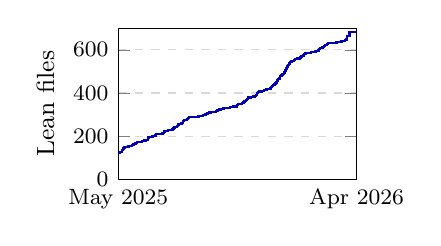
\begin{tikzpicture}
    \begin{axis}[
      width=0.38\textwidth,
      height=3.5cm,
      ymin=0, ymax=700,
      xmin=0, xmax=337.7,
      xtick={0,337.7},
      xticklabels={May 2025,Apr 2026},
      x tick label style={font=\footnotesize},
      ylabel={Lean files},
      ylabel style={font=\small},
      yticklabel style={font=\footnotesize},
      grid=major,
      grid style={dashed, gray!30},
      const plot,
    ]
    \addplot[blue!70!black, thick] coordinates {
        (0.00,122)
        (0.36,122)
        (0.42,122)
        (0.42,122)
        (0.43,122)
        (0.43,122)
        (0.45,122)
        (0.45,122)
        (0.46,122)
        (0.47,122)
        (0.48,122)
        (0.49,122)
        (0.50,122)
        (0.54,122)
        (0.62,122)
        (0.63,122)
        (0.64,122)
        (0.64,122)
        (0.68,122)
        (0.69,122)
        (0.71,122)
        (0.71,122)
        (0.72,122)
        (0.72,122)
        (0.72,122)
        (0.73,122)
        (1.37,122)
        (1.55,122)
        (1.66,122)
        (1.80,122)
        (1.94,122)
        (1.96,123)
        (1.97,124)
        (2.43,124)
        (2.44,124)
        (2.54,124)
        (2.75,125)
        (2.76,125)
        (3.92,126)
        (3.97,126)
        (4.54,126)
        (4.56,127)
        (4.60,127)
        (4.69,127)
        (4.74,128)
        (4.80,129)
        (5.43,129)
        (5.54,130)
        (5.55,131)
        (5.55,132)
        (5.57,133)
        (5.58,134)
        (5.84,135)
        (5.87,136)
        (5.95,136)
        (6.40,137)
        (6.46,138)
        (6.47,139)
        (6.51,139)
        (6.63,140)
        (6.68,140)
        (6.96,141)
        (7.38,142)
        (7.43,143)
        (7.51,143)
        (7.54,143)
        (7.65,144)
        (7.70,144)
        (8.41,144)
        (8.49,145)
        (8.62,146)
        (8.65,147)
        (8.71,148)
        (9.45,149)
        (9.46,149)
        (9.51,149)
        (9.72,149)
        (9.93,149)
        (10.72,149)
        (10.74,149)
        (11.89,149)
        (13.74,150)
        (13.79,151)
        (13.97,152)
        (14.52,153)
        (14.68,154)
        (15.40,154)
        (15.43,155)
        (15.58,155)
        (16.68,156)
        (19.50,157)
        (19.50,158)
        (20.43,158)
        (20.44,159)
        (20.54,160)
        (21.34,161)
        (21.55,162)
        (21.55,163)
        (22.54,164)
        (23.52,165)
        (23.58,166)
        (24.50,167)
        (26.45,168)
        (26.47,171)
        (27.60,172)
        (27.60,172)
        (28.73,172)
        (28.77,172)
        (29.54,172)
        (29.58,172)
        (29.60,172)
        (29.60,172)
        (29.69,172)
        (29.72,172)
        (29.73,172)
        (29.73,172)
        (29.79,173)
        (31.84,173)
        (31.84,174)
        (33.59,175)
        (33.59,176)
        (33.65,176)
        (34.87,177)
        (35.18,177)
        (35.39,177)
        (36.41,179)
        (36.97,179)
        (37.31,180)
        (37.43,180)
        (37.52,180)
        (39.58,181)
        (39.68,181)
        (41.44,182)
        (41.82,183)
        (42.52,183)
        (42.55,184)
        (42.63,184)
        (42.65,184)
        (42.71,194)
        (42.76,195)
        (42.87,195)
        (43.44,195)
        (43.45,195)
        (43.76,195)
        (44.40,195)
        (44.45,195)
        (44.45,195)
        (47.35,196)
        (47.56,197)
        (48.46,198)
        (48.64,198)
        (48.67,198)
        (49.49,199)
        (49.97,200)
        (50.37,200)
        (50.37,200)
        (50.47,200)
        (50.53,201)
        (51.64,202)
        (51.72,203)
        (52.66,204)
        (53.30,205)
        (53.43,206)
        (53.43,207)
        (53.44,208)
        (54.63,208)
        (55.29,209)
        (55.49,209)
        (55.49,210)
        (61.51,211)
        (62.70,212)
        (62.77,213)
        (63.43,215)
        (63.62,216)
        (64.38,217)
        (64.48,219)
        (64.51,219)
        (64.57,220)
        (64.65,220)
        (64.66,221)
        (64.74,221)
        (65.44,221)
        (65.46,222)
        (67.46,223)
        (67.56,224)
        (67.56,224)
        (68.47,225)
        (68.63,225)
        (68.72,225)
        (68.74,225)
        (68.79,225)
        (70.45,225)
        (70.50,225)
        (70.60,226)
        (70.63,227)
        (72.71,227)
        (74.58,228)
        (74.84,228)
        (74.84,228)
        (75.51,229)
        (75.57,229)
        (76.47,230)
        (76.67,231)
        (77.44,231)
        (77.54,232)
        (77.75,232)
        (77.75,232)
        (77.76,233)
        (77.76,233)
        (77.77,234)
        (77.79,234)
        (77.89,235)
        (78.45,235)
        (78.46,236)
        (78.47,236)
        (78.48,237)
        (78.60,238)
        (78.72,238)
        (78.87,238)
        (79.35,239)
        (79.66,240)
        (79.66,240)
        (79.73,241)
        (82.89,242)
        (83.38,244)
        (83.39,244)
        (83.40,245)
        (83.40,245)
        (83.51,245)
        (83.65,245)
        (83.69,248)
        (84.36,249)
        (84.56,250)
        (84.56,251)
        (84.66,252)
        (84.86,252)
        (84.86,253)
        (84.87,254)
        (85.38,254)
        (85.41,255)
        (85.68,255)
        (85.73,256)
        (86.29,256)
        (86.40,256)
        (86.40,256)
        (86.44,256)
        (87.44,257)
        (88.81,258)
        (90.35,259)
        (90.49,259)
        (90.52,259)
        (90.60,260)
        (91.40,260)
        (91.41,260)
        (91.41,261)
        (91.42,262)
        (91.43,263)
        (91.45,263)
        (91.46,264)
        (91.49,265)
        (91.52,266)
        (91.57,267)
        (91.62,267)
        (91.67,268)
        (91.72,269)
        (92.39,269)
        (92.42,269)
        (92.52,269)
        (92.59,269)
        (92.68,269)
        (92.75,269)
        (92.79,270)
        (92.90,270)
        (93.42,270)
        (93.44,271)
        (93.44,272)
        (93.66,272)
        (93.68,273)
        (96.45,273)
        (96.63,274)
        (96.65,274)
        (96.71,274)
        (96.76,274)
        (96.79,275)
        (96.94,276)
        (97.29,277)
        (97.31,278)
        (97.49,279)
        (98.44,279)
        (98.56,279)
        (98.65,280)
        (98.71,281)
        (98.78,282)
        (99.37,283)
        (99.44,284)
        (99.72,284)
        (100.47,284)
        (100.62,285)
        (100.64,286)
        (100.65,286)
        (100.74,286)
        (100.81,287)
        (100.82,288)
        (100.98,288)
        (101.15,288)
        (102.41,289)
        (103.39,289)
        (105.51,289)
        (105.53,289)
        (111.40,290)
        (113.35,291)
        (113.70,292)
        (118.79,293)
        (119.44,294)
        (119.62,294)
        (120.35,295)
        (120.36,296)
        (120.36,297)
        (120.52,297)
        (120.65,297)
        (120.69,298)
        (120.90,299)
        (123.35,300)
        (124.49,302)
        (124.77,303)
        (125.54,304)
        (125.61,305)
        (126.47,306)
        (127.33,307)
        (128.64,308)
        (128.66,309)
        (131.47,310)
        (131.47,311)
        (132.44,311)
        (134.55,311)
        (135.40,312)
        (136.51,313)
        (138.48,313)
        (138.49,313)
        (138.59,314)
        (138.63,315)
        (139.46,316)
        (139.49,317)
        (139.65,318)
        (140.55,319)
        (141.56,320)
        (142.48,321)
        (142.54,322)
        (142.57,322)
        (142.69,323)
        (145.51,324)
        (145.51,324)
        (145.51,324)
        (146.40,325)
        (146.45,326)
        (146.56,326)
        (146.60,327)
        (147.52,327)
        (147.56,327)
        (147.60,327)
        (147.63,327)
        (147.70,327)
        (147.73,327)
        (148.34,327)
        (148.36,327)
        (148.50,327)
        (148.71,327)
        (148.74,327)
        (148.75,328)
        (149.59,329)
        (149.60,330)
        (149.88,331)
        (152.72,331)
        (153.67,331)
        (153.94,331)
        (153.94,331)
        (153.94,331)
        (153.94,331)
        (153.94,331)
        (153.94,331)
        (153.94,331)
        (153.94,331)
        (154.37,332)
        (154.40,332)
        (154.40,332)
        (154.40,332)
        (154.40,332)
        (154.40,332)
        (154.41,332)
        (154.86,332)
        (158.65,333)
        (158.67,334)
        (159.44,334)
        (160.50,334)
        (160.55,335)
        (160.55,336)
        (162.49,336)
        (162.54,337)
        (162.61,337)
        (163.50,337)
        (163.63,337)
        (167.51,338)
        (167.53,339)
        (167.68,339)
        (167.68,339)
        (167.77,339)
        (167.78,339)
        (167.78,339)
        (167.86,339)
        (168.39,339)
        (168.41,340)
        (168.41,341)
        (168.41,342)
        (168.44,343)
        (168.46,344)
        (168.50,344)
        (168.50,344)
        (169.67,344)
        (169.68,345)
        (169.68,345)
        (169.76,346)
        (169.76,347)
        (169.79,348)
        (169.79,348)
        (169.90,350)
        (170.04,350)
        (174.63,350)
        (174.68,350)
        (174.99,351)
        (175.68,351)
        (175.71,352)
        (176.63,352)
        (176.63,352)
        (176.63,352)
        (176.63,352)
        (176.74,352)
        (176.76,352)
        (177.58,353)
        (177.58,353)
        (177.58,353)
        (177.58,353)
        (177.58,353)
        (177.58,353)
        (177.58,353)
        (177.60,353)
        (177.61,354)
        (177.61,355)
        (177.61,355)
        (177.61,355)
        (177.63,356)
        (177.66,357)
        (177.67,358)
        (177.83,359)
        (177.94,360)
        (179.44,360)
        (179.44,360)
        (179.57,360)
        (179.81,361)
        (179.88,362)
        (180.41,363)
        (180.46,363)
        (180.46,363)
        (180.46,363)
        (180.49,364)
        (180.52,365)
        (181.53,366)
        (181.59,367)
        (181.60,368)
        (181.63,369)
        (181.67,369)
        (181.95,370)
        (181.98,372)
        (182.57,373)
        (183.36,374)
        (183.41,375)
        (183.41,376)
        (183.49,376)
        (183.57,377)
        (183.60,378)
        (183.73,378)
        (184.54,378)
        (184.54,379)
        (188.48,379)
        (188.50,379)
        (188.57,380)
        (188.59,381)
        (188.89,382)
        (189.76,382)
        (190.51,383)
        (190.59,384)
        (190.79,384)
        (190.84,384)
        (190.84,384)
        (190.84,384)
        (190.84,384)
        (190.84,384)
        (190.88,384)
        (191.46,384)
        (191.85,384)
        (193.95,386)
        (193.95,386)
        (194.67,386)
        (195.71,387)
        (195.73,388)
        (195.73,389)
        (195.82,390)
        (195.83,390)
        (195.84,390)
        (195.88,390)
        (195.88,390)
        (195.89,390)
        (196.51,390)
        (196.53,391)
        (196.53,392)
        (196.54,393)
        (196.63,394)
        (196.64,395)
        (196.64,396)
        (196.64,397)
        (196.71,398)
        (196.81,399)
        (197.39,400)
        (197.40,400)
        (197.44,400)
        (197.62,401)
        (197.67,402)
        (197.88,403)
        (198.48,404)
        (198.56,405)
        (198.98,405)
        (199.34,405)
        (199.36,405)
        (199.48,405)
        (199.48,405)
        (199.48,405)
        (199.48,405)
        (199.75,406)
        (199.84,407)
        (201.01,407)
        (201.49,407)
        (201.51,407)
        (202.64,407)
        (203.60,408)
        (203.60,409)
        (203.77,410)
        (204.52,410)
        (206.66,411)
        (206.92,412)
        (206.95,413)
        (206.99,414)
        (208.80,414)
        (208.81,415)
        (208.94,416)
        (209.49,416)
        (209.50,416)
        (209.94,416)
        (210.42,417)
        (212.61,418)
        (214.53,419)
        (215.61,420)
        (215.71,421)
        (215.76,422)
        (215.82,422)
        (216.46,422)
        (216.46,423)
        (216.48,424)
        (216.62,424)
        (216.64,424)
        (216.64,424)
        (216.78,425)
        (216.81,426)
        (216.90,427)
        (216.97,427)
        (217.51,427)
        (217.58,428)
        (217.93,429)
        (218.42,430)
        (218.43,431)
        (218.78,431)
        (218.87,432)
        (219.43,433)
        (219.70,434)
        (219.70,436)
        (220.77,437)
        (220.77,438)
        (220.93,439)
        (221.34,440)
        (221.41,441)
        (221.82,442)
        (222.49,442)
        (222.49,442)
        (222.59,443)
        (222.65,444)
        (222.72,445)
        (222.97,445)
        (223.35,445)
        (223.36,445)
        (223.54,445)
        (223.54,446)
        (223.56,446)
        (223.62,446)
        (223.67,446)
        (223.79,446)
        (223.81,447)
        (223.94,448)
        (224.38,449)
        (224.38,449)
        (224.40,450)
        (224.42,450)
        (224.49,450)
        (224.50,451)
        (224.51,451)
        (224.51,451)
        (224.51,451)
        (224.53,451)
        (224.54,451)
        (224.54,451)
        (224.54,451)
        (224.54,451)
        (224.55,452)
        (224.58,453)
        (224.59,454)
        (224.59,454)
        (224.82,454)
        (225.29,455)
        (225.30,455)
        (225.40,456)
        (225.46,457)
        (225.54,457)
        (225.62,457)
        (225.74,458)
        (225.75,459)
        (225.77,460)
        (226.40,461)
        (226.56,461)
        (226.64,462)
        (226.66,462)
        (226.69,463)
        (226.79,463)
        (226.84,463)
        (226.84,463)
        (226.84,464)
        (226.85,465)
        (226.88,466)
        (227.77,466)
        (228.65,466)
        (228.65,467)
        (228.66,468)
        (228.76,469)
        (228.85,470)
        (228.96,471)
        (229.59,471)
        (229.62,472)
        (229.63,473)
        (229.65,474)
        (229.65,475)
        (229.66,476)
        (229.76,477)
        (229.77,477)
        (230.00,477)
        (230.38,478)
        (230.58,479)
        (230.64,480)
        (230.92,481)
        (231.72,482)
        (231.74,482)
        (231.76,482)
        (231.77,483)
        (231.85,483)
        (231.94,483)
        (231.95,484)
        (231.97,485)
        (232.46,485)
        (232.48,486)
        (232.73,487)
        (232.85,487)
        (232.85,487)
        (233.38,487)
        (233.41,487)
        (233.52,487)
        (233.67,487)
        (234.40,488)
        (234.86,489)
        (234.87,490)
        (234.88,490)
        (234.90,490)
        (234.91,490)
        (234.92,490)
        (234.97,490)
        (234.97,491)
        (234.97,492)
        (235.00,493)
        (235.31,493)
        (235.33,494)
        (235.37,495)
        (235.59,496)
        (235.64,497)
        (235.82,498)
        (235.83,499)
        (235.85,500)
        (236.43,501)
        (236.47,501)
        (236.52,502)
        (236.78,503)
        (236.78,504)
        (237.35,505)
        (237.38,506)
        (237.39,507)
        (237.41,508)
        (237.48,509)
        (237.61,510)
        (237.68,511)
        (237.74,512)
        (238.38,513)
        (238.39,514)
        (238.45,514)
        (238.51,514)
        (238.71,515)
        (238.89,515)
        (238.91,515)
        (238.93,516)
        (239.35,516)
        (239.40,517)
        (239.43,519)
        (239.43,520)
        (239.47,521)
        (239.52,522)
        (239.72,522)
        (239.75,522)
        (239.76,523)
        (239.79,524)
        (239.82,525)
        (239.88,525)
        (239.95,525)
        (240.35,526)
        (240.71,527)
        (240.72,528)
        (240.73,529)
        (240.73,530)
        (240.84,530)
        (241.50,530)
        (241.58,530)
        (241.83,530)
        (241.84,531)
        (242.37,532)
        (242.38,533)
        (242.60,533)
        (242.64,534)
        (242.64,535)
        (242.64,536)
        (242.68,537)
        (243.32,538)
        (243.37,538)
        (243.47,539)
        (243.52,540)
        (243.59,541)
        (243.74,542)
        (244.00,543)
        (244.00,543)
        (244.33,543)
        (244.34,543)
        (244.70,544)
        (245.39,545)
        (245.49,546)
        (245.49,546)
        (245.91,547)
        (245.91,548)
        (246.74,548)
        (246.79,548)
        (246.93,549)
        (246.95,549)
        (247.54,549)
        (248.32,549)
        (248.35,549)
        (248.44,549)
        (248.48,549)
        (248.54,549)
        (249.60,550)
        (249.62,551)
        (249.88,552)
        (249.89,552)
        (250.33,553)
        (250.33,554)
        (250.41,555)
        (250.41,556)
        (250.43,556)
        (250.43,556)
        (250.44,556)
        (250.44,556)
        (251.37,556)
        (251.37,556)
        (251.37,556)
        (251.37,556)
        (251.38,556)
        (251.39,556)
        (251.39,556)
        (251.46,557)
        (251.53,557)
        (251.72,558)
        (251.85,558)
        (251.85,558)
        (251.86,558)
        (251.86,558)
        (251.86,558)
        (251.86,558)
        (251.87,558)
        (252.42,558)
        (252.42,558)
        (252.42,558)
        (252.42,558)
        (252.42,558)
        (252.42,558)
        (252.43,558)
        (252.65,558)
        (252.78,558)
        (253.37,558)
        (253.41,558)
        (253.42,558)
        (253.43,558)
        (253.44,559)
        (253.47,559)
        (253.63,559)
        (253.63,560)
        (253.71,561)
        (253.72,556)
        (253.72,556)
        (253.73,557)
        (253.92,557)
        (254.52,558)
        (254.60,560)
        (254.89,560)
        (256.89,561)
        (256.91,562)
        (257.37,562)
        (257.39,562)
        (257.43,562)
        (257.45,563)
        (257.46,564)
        (257.66,564)
        (258.42,564)
        (258.46,564)
        (258.54,564)
        (258.54,564)
        (258.55,564)
        (258.58,564)
        (258.61,564)
        (258.84,565)
        (259.38,566)
        (259.50,567)
        (259.50,568)
        (259.51,569)
        (259.52,569)
        (260.33,569)
        (260.33,570)
        (261.33,571)
        (261.36,571)
        (261.36,571)
        (261.55,572)
        (261.71,573)
        (261.79,574)
        (262.42,575)
        (262.60,576)
        (262.73,576)
        (262.81,577)
        (262.86,578)
        (263.69,579)
        (263.69,580)
        (263.70,580)
        (263.74,581)
        (264.54,581)
        (264.60,581)
        (264.66,582)
        (264.67,582)
        (264.67,582)
        (265.37,582)
        (265.50,583)
        (265.65,584)
        (265.79,584)
        (266.36,584)
        (267.45,584)
        (267.46,584)
        (267.61,584)
        (267.76,584)
        (268.45,584)
        (270.28,584)
        (271.40,585)
        (271.40,585)
        (271.42,585)
        (271.61,585)
        (272.00,586)
        (272.73,586)
        (273.42,586)
        (273.45,586)
        (273.49,587)
        (273.50,587)
        (273.60,588)
        (273.63,588)
        (273.63,589)
        (273.74,589)
        (274.48,589)
        (274.51,589)
        (274.68,589)
        (275.34,589)
        (275.38,589)
        (276.99,589)
        (277.55,589)
        (277.73,589)
        (277.88,589)
        (277.90,589)
        (278.46,589)
        (278.46,589)
        (278.60,591)
        (278.79,591)
        (279.48,591)
        (279.58,591)
        (279.66,592)
        (279.67,592)
        (279.73,593)
        (280.35,593)
        (280.38,594)
        (280.38,594)
        (280.54,594)
        (280.55,594)
        (280.60,594)
        (281.35,594)
        (281.49,594)
        (281.59,595)
        (281.70,595)
        (281.74,596)
        (283.38,597)
        (283.39,597)
        (284.34,598)
        (284.34,599)
        (284.35,600)
        (284.35,600)
        (284.37,601)
        (284.56,601)
        (284.89,602)
        (284.89,603)
        (284.95,604)
        (284.96,605)
        (285.35,605)
        (285.38,606)
        (285.40,607)
        (285.42,607)
        (285.42,607)
        (285.68,608)
        (285.77,609)
        (286.30,609)
        (286.83,609)
        (287.39,609)
        (287.64,609)
        (288.68,610)
        (288.69,611)
        (289.34,611)
        (289.53,611)
        (289.53,611)
        (289.54,611)
        (289.54,611)
        (289.54,611)
        (289.54,611)
        (289.54,611)
        (289.54,611)
        (289.54,611)
        (289.54,611)
        (289.54,611)
        (289.54,611)
        (289.54,611)
        (289.54,611)
        (289.54,611)
        (289.54,611)
        (289.54,611)
        (289.54,611)
        (289.54,611)
        (289.54,611)
        (289.54,611)
        (289.55,611)
        (289.55,611)
        (289.55,611)
        (289.56,611)
        (289.59,611)
        (289.59,611)
        (289.59,612)
        (289.59,612)
        (289.63,612)
        (289.68,612)
        (289.73,612)
        (289.74,612)
        (289.91,612)
        (289.94,612)
        (289.97,612)
        (290.47,612)
        (290.59,612)
        (290.74,612)
        (291.44,613)
        (291.47,614)
        (291.47,614)
        (291.65,615)
        (291.95,616)
        (292.33,616)
        (292.33,617)
        (292.33,618)
        (292.46,618)
        (292.52,618)
        (293.36,619)
        (293.38,619)
        (293.44,620)
        (293.44,621)
        (293.48,621)
        (293.76,622)
        (293.85,623)
        (293.89,624)
        (293.98,624)
        (294.40,624)
        (294.79,624)
        (295.31,624)
        (295.36,624)
        (295.56,624)
        (295.57,624)
        (295.98,625)
        (295.98,626)
        (295.98,627)
        (295.99,628)
        (296.73,628)
        (296.81,628)
        (296.83,628)
        (297.40,628)
        (297.59,628)
        (297.64,630)
        (297.65,630)
        (298.56,631)
        (299.35,632)
        (299.43,632)
        (299.70,632)
        (299.97,632)
        (300.38,632)
        (300.48,632)
        (300.51,632)
        (300.92,633)
        (301.40,633)
        (302.35,633)
        (302.57,633)
        (302.77,633)
        (303.89,633)
        (303.92,633)
        (304.62,633)
        (306.50,633)
        (306.54,633)
        (307.62,633)
        (308.44,634)
        (308.90,634)
        (309.28,634)
        (309.36,634)
        (310.52,635)
        (311.86,635)
        (311.87,635)
        (311.87,635)
        (311.88,636)
        (311.90,637)
        (311.92,637)
        (311.92,637)
        (313.58,637)
        (314.54,637)
        (314.67,637)
        (314.81,637)
        (315.73,638)
        (317.31,639)
        (317.32,641)
        (317.76,641)
        (319.93,641)
        (319.93,641)
        (319.93,641)
        (319.93,641)
        (319.93,641)
        (319.93,641)
        (319.93,641)
        (319.95,641)
        (319.98,641)
        (320.10,642)
        (320.32,642)
        (320.37,642)
        (320.39,642)
        (320.40,642)
        (320.41,642)
        (320.41,642)
        (320.41,642)
        (320.43,642)
        (320.43,642)
        (320.45,642)
        (320.58,642)
        (320.60,642)
        (320.71,642)
        (320.72,642)
        (320.74,642)
        (321.30,643)
        (321.38,644)
        (321.92,644)
        (322.26,644)
        (322.37,645)
        (322.63,645)
        (322.63,645)
        (322.63,645)
        (322.63,645)
        (322.88,645)
        (322.92,646)
        (322.95,646)
        (323.01,647)
        (323.34,647)
        (323.35,648)
        (323.35,648)
        (323.43,649)
        (323.56,650)
        (323.72,651)
        (323.73,652)
        (323.73,653)
        (323.73,654)
        (323.79,655)
        (323.87,656)
        (323.88,657)
        (323.95,658)
        (324.31,660)
        (324.43,661)
        (324.43,662)
        (324.59,663)
        (324.89,664)
        (325.94,664)
        (327.48,666)
        (327.72,681)
        (328.34,681)
        (329.59,681)
        (329.85,681)
        (330.55,681)
        (331.47,681)
        (331.47,681)
        (331.52,681)
        (331.56,681)
        (331.57,681)
        (331.66,681)
        (331.67,681)
        (331.69,681)
        (331.70,681)
        (334.57,681)
        (334.57,681)
        (334.57,681)
        (334.57,681)
        (334.66,681)
        (334.69,681)
        (334.77,681)
        (334.82,681)
        (334.96,681)
        (334.97,681)
        (335.46,681)
        (335.63,681)
        (335.69,681)
        (335.69,681)
        (335.70,681)
        (335.71,681)
        (335.71,681)
        (335.74,682)
        (335.77,682)
        (335.78,682)
        (335.78,682)
        (335.79,682)
        (335.96,682)
        (335.96,682)
        (335.96,682)
        (336.39,682)
        (336.53,682)
        (336.53,682)
        (336.56,681)
        (336.62,684)
        (336.64,684)
        (336.85,684)
        (337.43,684)
        (337.50,684)
        (337.50,684)
        (337.60,684)
        (337.69,684)
    };
    \end{axis}
  \end{tikzpicture}
  \vspace{-10pt}
  \caption{Repository growth over time.}
  \label{fig:repo_growth}
  \vspace{-15pt}
\end{wrapfigure}



The benchmark's problems are sourced from diverse mathematical literature for broad coverage.
Key sources include the collection of problems posed by Paul Erd\H{o}s, as catalogued on \emph{erdosproblems.com} \citep{erdosproblems}; the Kourovka Notebook of unsolved problems in group theory \citep{kourovka}; the IQOQI Vienna list of open quantum problems \citep{oqp}; well-known Wikipedia conjectures; conjectures from recent publications in academic journals and on arXiv; and questions asked on MathOverflow.
The number of problems per informal source is in Figure \ref{fig:benchmark_pipeline}.
Furthermore, the repository has grown steadily since its initial open-source release, as visualized in Figure \ref{fig:repo_growth}.


The collection is divided into two primary categories: \textbf{Unsolved Conjectures}, open research problems where a formal or informal proof would represent a new mathematical discovery; and \textbf{Solved Problems}, established theorems with known \emph{informal} proofs that benchmark an AI's ability to formalize existing arguments, though only a fraction currently have a \emph{formal} proof available.
We include both categories not only because they independently serve as benchmarks for different tasks (proof generation and auto-formalization), but also because they are often intertwined.
When formalizing an open conjecture, it is natural to also state and prove simpler, solved variations.
For instance, a general conjecture about the existence of Hadamard matrices of size $4k$ for all valid $k \in \mathbb{N}$ can be presented alongside the solved cases (e.g., for all $k \le 166$) and the first open case ($k = 167$).


Other sources of \emph{solved} problems are collections of conjectures that include both open and solved questions. In those cases, we also formalize the statements of the solved cases. They are often related in subject to the open conjectures, and hence the formalization of their statements and the auto-formalization of their proofs support the open conjectures.


The collection of solved problems also includes simpler statements, ranging from trivial to textbook level, which help validate the correctness of the underlying formalizations.
Including such simpler problems helps detect incorrect formalizations of open problems: a disproof of an easy special case or known variant might indicate that some of the definitions used have been stated incorrectly.
See below for examples of how those initial misformalizations can lead to improved formal and informal problem statements.
We strive to always state the simplest open variant of a conjecture, as well as the conjecture in greater generality.

\paragraph{The \lstinline{@[category]} attribute.}
To help navigate this collection, each statement is labeled with one of the following category tags: \lstinline[language={}]{research open} (an open research-level problem), \lstinline[language={}]{research solved} (a solved research-level problem), \lstinline[language={}]{textbook} (a textbook-level math problem ranging from high school to graduate level), \lstinline[language={}]{API} (statements developing foundational theory for a new definition intended for general reuse), and \lstinline[language={}]{test} (a statement serving as a sanity check).
The distribution of all categories is in Figure \ref{fig:benchmark_pipeline} on the right.



\paragraph{The \lstinline{@[subject]} attribute.}
Statements are also labeled with subject tags following the AMS Mathematics Subject Classification \citep{ams2020}.
The distribution by source collection and AMS subject classification is shown in Tables~\ref{tab:problems-by-collection} and~\ref{tab:ams-breakdown} (Appendix~\ref{sec:app_source_ams_tables}).
While number theory and combinatorics account for over half of all statements, the benchmark already spans over 10 AMS subjects (e.g., also quantum theory, or algebraic geometry), which we aim to broaden further.

\subsection{Formalization Methodology}\label{sec:formalization-methodology}

\begin{figure}[t!]
    \centering
    \begin{leancode}
/--
There are no indecomposable vector bundles of rank 2 on $\mathbb{P}^n$ for $n \ge 7$.
-/
@[category research open, AMS 14]
theorem hartshorne_conjecture (n : ℕ) (hn : 7 ≤ n)
    (F : VectorBundles (ProjectiveSpace (Fin (n + 1)) (Spec (.of ℂ))))
    (hF : F.rank = 2) : Nonempty (F.Splitting (Fin 2)) := by
  sorry
    \end{leancode}
    \caption{A statement in Formal Conjectures, an open conjecture from \citep{hartshorne1974varieties}. It includes an informal statement as a comment, tags, and a Lean statement.}
    \label{fig:example-statement}
\end{figure}

All problems are presented as Lean theorems with informal statements. While our core goal is providing open statements with \lstinline{sorry} placeholders for AI solvers to replace, we also include solved variants of conjectures and items from problem lists. For open problems, no proofs are provided. For solved items, we appreciate very short proofs or counterexamples (under 25--50 lines) that test the definitions. Longer proofs are excluded to keep the repository lightweight; instead, contributors are encouraged to host proofs in their own repositories and link to them using the \lstinline{@[formal_proof]} mechanism described below.

We provide an example statement in Figure \ref{fig:example-statement}.






\paragraph{The \texorpdfstring{\lean{answer(sorry)}}{answer(sorry)} mechanism.}
Many mathematical problems ask not just for a proof but for a specific \emph{answer}: a number, a function, or a set.
To handle this, we introduce an \lean{answer(sorry)} construct, implemented as a custom Lean term elaborator, that separates the task of discovering a computable answer from proving it correct.
For example, \enquote{What is the smallest $n$ such that $P(n)$?} is formalized with \lean{answer(sorry)} as a placeholder that a solver must replace with a concrete value, reducing the problem to a verifiable proof obligation.
The construct also handles unknown truth values: when \lean{answer(sorry)} appears in a biconditional, a solver replaces it with \lean{True} or \lean{False} to conjecture or refute a proposition.
See Appendix~\ref{sec:app_answer_sorry} for detailed examples and the full elaboration semantics.



\paragraph{The \enquote{for Mathlib} pattern.}
The project maintains a \texttt{FormalConjecturesForMathlib} directory containing 88 files of auxiliary definitions and lemmas not yet in Mathlib but needed for conjectures.
These results are asynchronously contributed upstream to Mathlib.
See Appendix~\ref{sec:app_for_mathlib} for details on the rationale and contents of this directory.


\paragraph{The \lstinline{@[formal_proof]} attribute.}
To keep the repository lightweight, the \lstinline{@[formal_proof]} attribute decouples problem statements from their solutions.
It supports three modes: (1)~\lean{formal_conjectures} for proofs solving exactly the type of the statement given here; it should point to a commit on top of a commit in the \texttt{main} branch of our repo, filling in the \lean{sorry};
(2)~\lstinline{lean4} for equivalent problems solved in Lean~4 elsewhere (e.g., in Mathlib or external repos); and
(3)~\lstinline{other_system} for problems solved in other systems like Lean~3, Isabelle, or Rocq.
This design links to external verification sources while keeping the repository maintainable.
The attribute applies to any solved category, though usage on a \lstinline{research open} problem triggers a linter warning.
Table~\ref{tab:formal_proof_baseline} summarizes proof coverage recorded via this attribute.

\subsection{Misformalizations}
\label{sec:misform}

It is notoriously difficult to formalize a mathematical problem \emph{correctly} without providing a formal proof.
A \emph{misformalization} is a formal statement that is incorrect.
To provide a rigorous foundation for benchmark quality, we introduce a taxonomy of misformalizations.
It includes the following levels, where in all cases the formal statement is incorrect.
\begin{enumerate}
    \item \textbf{Translation}: the informal statement is accurate and explicitly phrased.
    \item \textbf{Underspecified}: the informal statement is accurate but lacks detail.
    \item \textbf{Source}: the informal statement is not as intended.
\end{enumerate}


These levels are ordered with respect to the degree of contribution from the formalizer.
Level 1 misformalizations arise from the formalization only, while level 3 misformalizations arise from the informal text only.
Moreover, for a Lean expert who does not necessarily have domain expertise in the informal statements, levels are ordered with respect to difficulty to fix.
Note that level 2 and 3 misformalizations have been useful in clarifying informal statements in the literature.
An illustrative example is Erd\H{o}s Problem~978: multiple attempts to formalize the statement led to a refinement of the original informal problem\footnote{\url{https://www.erdosproblems.com/forum/thread/978}}.
The original statement,
\enquote{Are there infinitely many $n$ for which $f(n)$ is $(k-2)$-power-free?},
was found to require multiple additional hypotheses and became:
\enquote{If $k>3$, and for all primes $p$ there exists $n$ such that $p^{k-2}\nmid f(n)$, then are there infinitely many $n$ for which $f(n)$ is $(k-2)$-power-free?}
More broadly, informal texts may exclude trivial cases without explicitly describing them, while formalization requires these to be explicit.

Misformalizations can further be categorized into six types across the three levels: \emph{syntactic}, \emph{semantic}, and \emph{misrepresentation} errors at the translation level; \emph{implicit conventions} at the underspecified level; and \emph{reporting} and \emph{mathematical} errors at the source level.
The full taxonomy with definitions and representative pull requests is given in Appendix~\ref{sec:app_misform_taxonomy}.
Across the repository a total of $291$ misformalizations have been fixed, with \emph{misrepresentation} (48\%) and \emph{semantic} (35\%) errors being the most common (Table~\ref{tab:misform_table}).
Detailed code diffs illustrating these misformalization examples can be found in Appendix~\ref{sec:app_misformalization_examples}.

\subsection{Avoiding Misformalizations}
\label{sec:avoiding_misform}

\begin{figure}[t!]
    \centering
    \resizebox{\textwidth}{!}{%
        \begin{tikzpicture}[
    % Reduced vertical distance (0.6cm) and horizontal (1.2cm)
    node distance=0.6cm and 1.2cm,
    font=\sffamily,
    % Reduced minimum height to 1.2cm and inner sep to 6pt for vertical compactness
    flowbox/.style={rectangle, fill=#1!5, draw=#1!60!black, very thick, rounded corners=1.5ex, text width=3.6cm, minimum height=1.2cm, inner sep=6pt, align=center},
    % Arrow styles
    arrow/.style={thick, color=black!60, -{Stealth[scale=1.1]}},
    feedback/.style={thick, color=red!70!black, dashed, -{Stealth[scale=1.1]}},
    success/.style={thick, color=green!60!black, -{Stealth[scale=1.1]}},
    % Label styles (tightened inner sep)
    pathlabel/.style={font=\sffamily\scriptsize, text=black!80, align=center, fill=white, fill opacity=0.8, text opacity=1, inner sep=2pt, rounded corners=0.4ex}
]

    % ==========================================
    % ROW 1: The Forward Pipeline
    % ==========================================
    \node (source) [flowbox=green] {
        \textbf{Informal Source}\\[0.3ex]
        \color{black!70}\scriptsize Erdős, arXiv, etc.
    };

    \node (formalize) [flowbox=orange, right=of source] {
        \textbf{Human Formalization}\\[0.3ex]
        \color{black!70}\scriptsize Draft Lean~4 code \& tests
    };

    \node (repo) [flowbox=cyan, right=of formalize] {
        \textbf{Merge to Repository}\\[0.3ex]
        \color{black!70}\scriptsize \texttt{formal-conjectures}
    };


    % ==========================================
    % ROW 2: The Evaluation & Feedback Loop
    % ==========================================
    \node (eval) [flowbox=purple, below=of repo] {
        \textbf{Automated Runs}\\[0.3ex]
        \color{black!70}\scriptsize AI systems attempt proofs
    };

    \node (inspect) [flowbox=gray, below=of formalize] {
        \textbf{Verification \& Triage}\\[0.3ex]
        \color{black!70}\scriptsize Manual inspection of results
    };

    \node (status) [flowbox=cyan, below=of source] {
        \textbf{Status Updated}\\[0.3ex]
        \color{black!70}\scriptsize In repo \& informal source
    };


    % ==========================================
    % ROUTING ARROWS
    % ==========================================
    % 1. Forward Path
    \draw [arrow] (source.east) -- (formalize.west);
    \draw [arrow] (formalize.east) -- (repo.west);
    \draw [arrow] (repo.south) -- (eval.north);

    % 2. Into Triage
    \draw [arrow] (eval.west) -- (inspect.east) node[midway, pathlabel] {Proofs \&\\Disproofs};

    % 3. Feedback Loops (Red Dashed)
    \draw [feedback] (inspect.north) -- (formalize.south) node[midway, pathlabel] {Misformalization};

    % External Community Feedback (Diagonal)
    \draw [thick, dashed, color=black!50, -{Stealth[scale=1.1]}] (inspect.north west) -- (source.south east) node[midway, pathlabel, sloped] {Source Error};

    % 4. Success Path (Green)
    \draw [success] (inspect.west) -- (status.east) node[midway, pathlabel] {Valid \\ Result};

\end{tikzpicture}%
    }%
    \caption{Iterative pipeline for Formal Conjectures. Formalized statements are tested by periodic AI runs, solving problems or triggering a revision loop.}
    \label{fig:formalization_process}
\end{figure}

In Formal Conjectures, every contribution undergoes mandatory code review by humans with both Lean expertise and relevant mathematical domain knowledge.
While early contributions to the repository were written entirely by hand, the authoring process has evolved: most recent submissions use AI tooling, including agentic coding assistants and auto-formalization systems.
To facilitate high-quality AI-assisted contributions, the repository provides an \texttt{AGENTS.md} file with structured guidance for these tools.
Similarly, the review process increasingly leverages AI: reviewers use language models to cross-check formalizations against informal sources, and AlphaProof runs on submissions to catch potential misformalizations before merging.

Beyond this review process, we employ a number of additional strategies to mitigate the risk of misformalizations across the dataset.
Firstly, we employ and encourage a test-based design for definitions.
Any new definitions introduced should be accompanied by a suite of proven \texttt{test} lemmas and \texttt{API} statements that are designed to establish
expected behavior of the definition and mitigate the risk of edge-case errors.
Lean and \lstinline{Mathlib}'s tooling (for example \lstinline{decide}) can be employed to prove many of these \texttt{test} statements.
As of the \href{https://github.com/google-deepmind/formal-conjectures/releases/tag/bench-v1-lean4.27.0}{\texttt{bench-v1-lean4.27.0} release}, the repository contains \fcCountTest{} \texttt{test} statements and \fcCountAPI{} \texttt{API} statements, amounting to \fcCountInfraPct\% of the repository statements.

Secondly, automated theorem provers like AlphaProof regularly attempt proofs and disproofs across the repository (Figure \ref{fig:formalization_process}); manually inspecting these results primarily reveals misformalizations.
In contrast to test-based design, which proactively reduces the risk of edge-case errors, this retroactive approach is capable of unearthing misformalizations across all categories as described in Section~\ref{sec:misform}.
In addition, we use Gemini, AlphaProof, and other tools to automatically cross-check formalizations against their informal source texts, flagging potential discrepancies for human review.
Future work involves further automating these processes in GitHub CI in order to reduce the overhead of manual post-hoc fixes from the maintainers.

Thirdly, custom Lean linters built on Mathlib's framework enforce metadata and documentation standards across contributions.
These cover AMS classification tags, \lstinline{answer(sorry)} usage, problem category annotations, and module docstrings.

Finally, as Formal Conjectures has grown in stature, community engagement and proof/disproof attempts from external automated theorem provers have been increasingly valuable.
Furthermore, insights and corrections discovered through this process are actively upstreamed to the original sources, e.g., prompting the maintainer of the Erdős problems website to regularly clarify and adjust the informal problem statements.
